\lab{Optimal Reentry of a Spacecraft}{Optimal Reentry of a Spacecraft}
\label{lab:reentry}
\objective{
We look at two problems related to space flight: The second problem is to choose the optimal path for reentry into the atmosphere, where the total heating experienced by the craft is minimized. 
}


We begin by giving the control system that describes the path of the vehicle through the atmosphere
\footnote{This control problem and its numerical solution are thoroughly described in 'Introduction to Numerical Analysis' by J. Stoer, R. Bulirsch (pg 524). 
We will mirror their presentation throughout this lab.}. 
If $v$ is the velocity of the spacecraft, $\gamma$ is the angle of the flight path, $\xi$ is the normalized altitude above the Earth's surface ($\xi = h/R$, where $R$ is the radius of the Earth and $h$ the altitude of the spacecraft above the Earth), and $u$ is the control variable that represents the angle of attack of the spacecraft, the flight path can be described by 
\begin{align}
\begin{split}
v' &= -s\rho v^2C_D(u) - \frac{g\sin(\gamma)}{(1+\xi)^2},\\
\gamma ' &= s \rho v C_L(u) + \frac{v \cos(\gamma)}{R(1+\xi)} - \frac{g \cos \gamma}{v(1+\xi)^2},\\
\xi' &= \frac{v \sin \gamma}{R}.
\end{split} \label{eqn:reentry:control_system}
\end{align}
$C_D$ and $C_L$ represent drag and lift coefficients, and are functions of the angle of attack $u$: $C_D(u) = 1.174 - .9\cos u$, $C_L(u) = 0.6\sin u$. 
The atmospheric density is represented by $\rho = \rho_0e^{-R\beta\xi}$, where  $\rho_0$ is the atmospheric density at the surface of the earth. 
Parameter $s = \frac{1}{2}S/m$, where $S$ is the frontal area of the craft and $m$ is its mass, and $g$ represents the force of gravity. 
The numerical values we will use are $g = 3.2172\times10^{-4}$, $s = 26,600$, $R = 209$ $(209\times 10^5 \text{ ft})$, $\beta = 4.26$ and $\rho_0 = 2.704\times 10^{-3}$.
The trajectory of the spacecraft must also satisfy the boundary conditions
\begin{align}
\begin{split}
	v(0) &= 0.36 \quad (36000 \text{ ft/sec}),\\
	\gamma(0) &= -8.1^\circ \frac{\pi}{180^\circ}, \\
	\xi(0)&= \frac{4}{R}\quad (h = 400000 \text{ ft}), \\
	v(T) &= 0.27,\\
	\gamma(T) &= 0, \\
	\xi(T)&= \frac{2.5}{R}, \\
\end{split}
\end{align}
where $T$ represents the time at the end of the reentry maneuver. 


We consider the problem of choosing the path of reentry for a spacecraft, so as to minimize the total heating of the craft. 
The functional describing the total heating is 
\[
J[u] = \int_0^T 10v^3 \sqrt{\rho}.
\]
To simpify notation, we rewrite \eqref{eqn:reentry:control_system} in the form $y' = G(y)$, where $y = [y_0, y_1, y_2]^T=[v,\gamma, \xi]^T$ and $G$ has component functions $G = [G_0, G_1, G_2]^T$. The Hamiltonian for this control system is given by 
\begin{align}
H &=  10v^3 \sqrt{\rho} + p_0G_0 + p_1G_1 + p_2G_2,
\end{align}
where $p = [p_0,p_1,p_2]^T$ is the adjoint variable. 
The optimal state and adjoint equations are thus given by 
\begin{align}
	\dot{y} &= H_{p},\\
	\dot{p} &= -H_{y} \label{eqn:reentry:adjoint_system}
\end{align}

To our boundary conditions we add the terminal condition that $H = 0$ at $t = T$.
% \footnote{BNDSCO - A program for the numerical solution of optimal control problems, H.J. Oberle and W. Grimm, 1989}

\begin{figure}
\centering
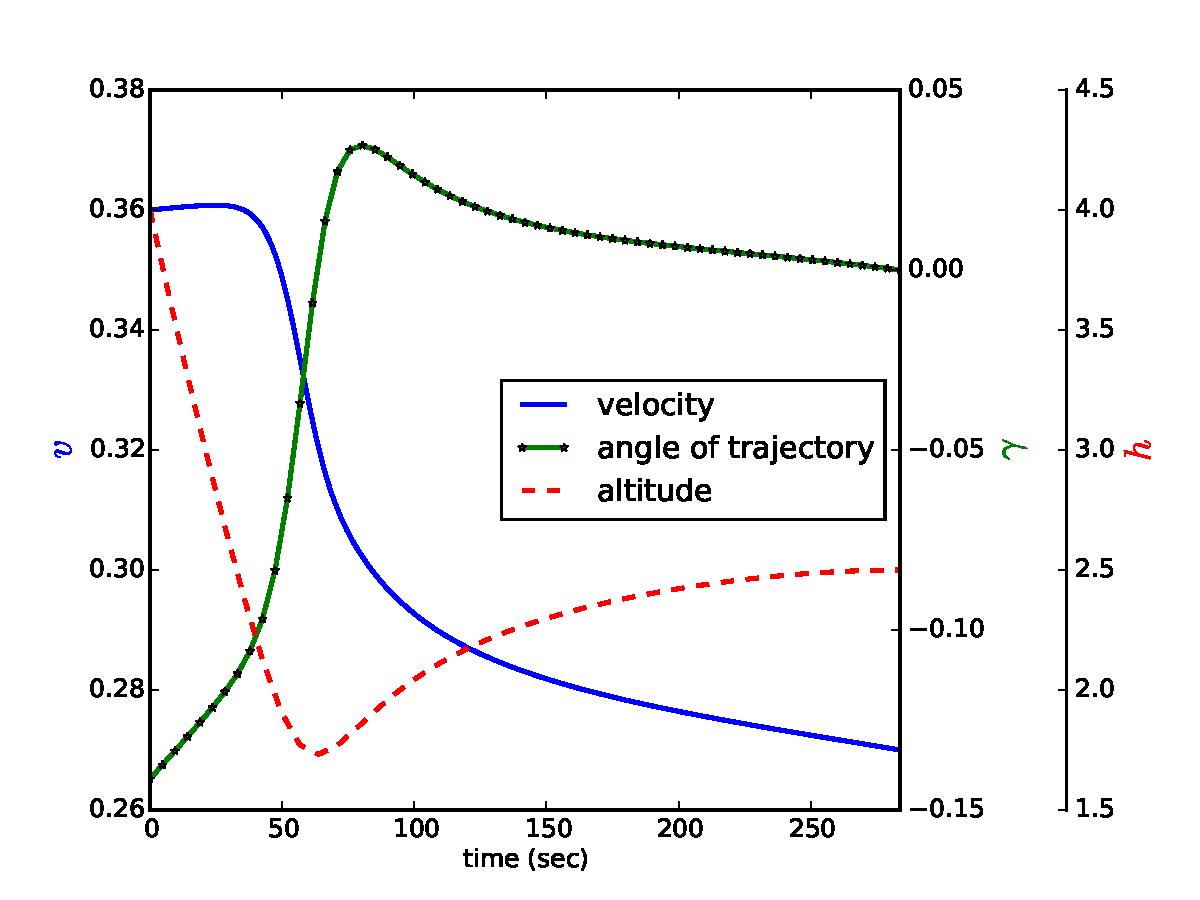
\includegraphics[width=\textwidth]{solutions.pdf}
\caption{The solution of ?%\eqref{reentry:solutions}.
}
\label{fig:reentry:solutions}
\end{figure}



\section*{Constructing an Initial Guess}
Most BVP solvers require an equal number of differential equations and boundary conditions. Currently we have 6 ODEs and 7 boundary conditions. 

Difficulties with the bvp include providing an initial guess that is sufficiently close to the solution.  Since this is a sensitive problem, we will use a heuristic method to help us find a good initial guess.





% \begin{figure}
% \begin{minipage}[b]{.47\linewidth}
% \centering
% 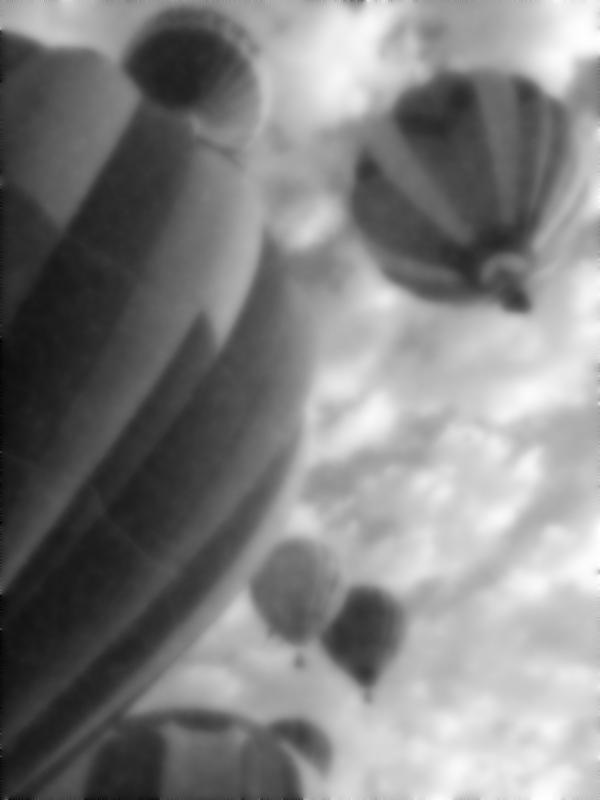
\includegraphics[width=\textwidth]{diffusion_denoised_baloons_resized_bw.jpg}
% \caption*{Initial diffusion-based approach}
% \end{minipage}
% \hspace{0.5cm}
% \begin{minipage}[b]{0.47\linewidth}
% \centering
% 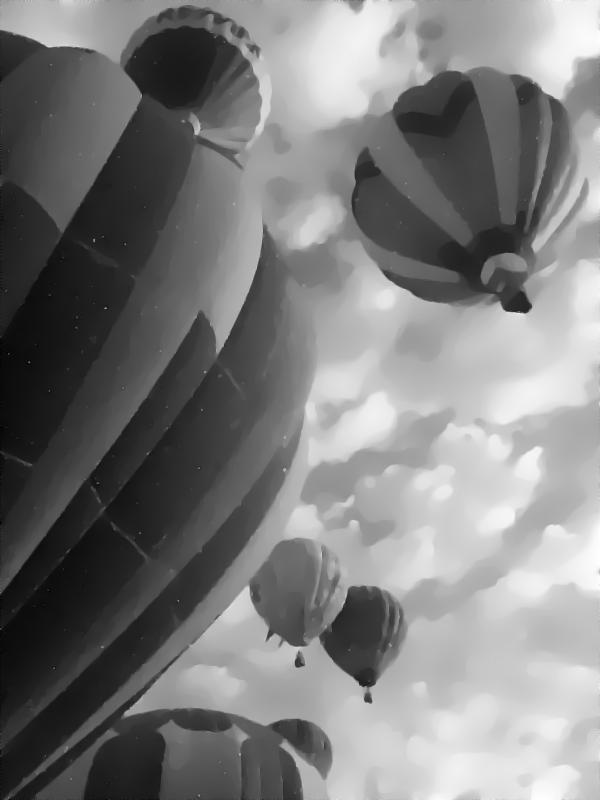
\includegraphics[width=\textwidth]{tv_denoised_baloons_resized_bw.jpg}
% \caption*{Total variation based approach}
% \end{minipage}
% \caption{The solutions of \eqref{tv_images:diffusion_flow} and \eqref{tv_images:tv_flow}, found using a first order Euler step in time and centered differences in space.}
% \label{fig:noise_compare_attempts}
% \end{figure}



% \begin{align}
% \begin{split}
% \end{split} \label{reentry:label}
% \end{align}
%
%
% \begin{problem}
%
% \begin{lstlisting}
% \end{lstlisting}
% \end{problem}


% \begin{figure}
% \centering
% 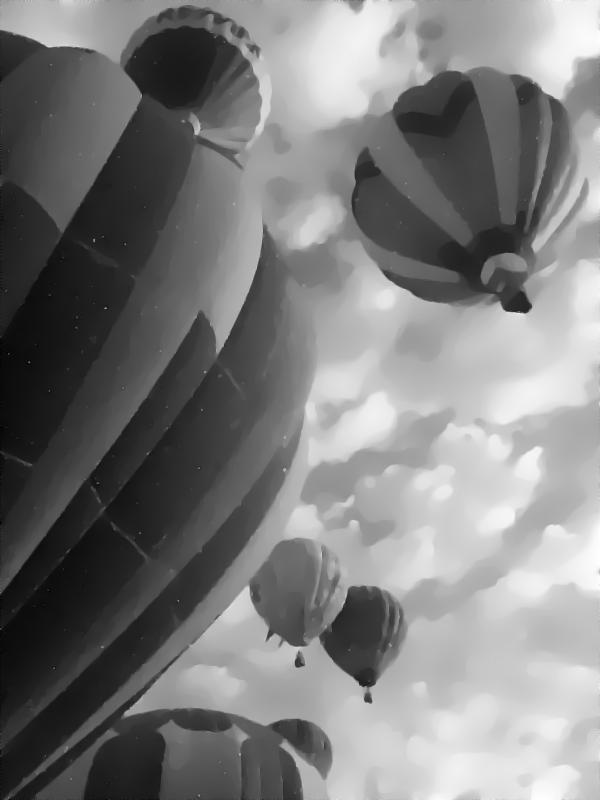
\includegraphics[width=6cm]{tv_denoised_baloons_resized_bw.jpg}
% \caption{The solution of \eqref{tv_images:diffusion_flow}, found using a first order Euler step in time and centered differences in space.}
% \label{fig:tv_image_denoised}
% \end{figure}







